\documentclass[nofilelist]{cslthse-msc}
% to show a list of used packages at the end of the document, delete the nofilelist option
%\documentclass{cslthse-msc}
\usepackage[utf8]{inputenc}
\usepackage[english]{babel}
\usepackage{amsmath}
%\usepackage{amsfonts}
%%\usepackage{amssymb}
\usepackage{amsthm}
%\usepackage{makeidx}
\usepackage{graphicx}
\usepackage[titletoc, header, page]{appendix}
\usepackage{transparent}

% used to display the used files at the end. Select nofilelist as a package option to disable this
\listfiles % initialize

%\geometry{showframe}
%better like this?
\student{Nicholas Boyd Isacsson}{nicholas@isacsson.se}
%\students{Flavius Gruian}{Flavius.Gruian@cs.lth.se}{Camilla Lekebjer}{Camilla.Lekebjer@cs.lth.se}

\thesisnumber{LU-CS-EX: 2023-79} % Magic Number! Do not change unless Birger Swahn asks you to do so!
% default is Master. Uncomment the following for "kandidatarbete"/Bachelor's thesis
%\thesistype{Bachelor}{Kandidatarbete}

%\title{Formatting a Master's Thesis}
\title{Typechecker Generation using Reference Attribute Grammars}
\svensktitel{Infoga den Svenska titeln här!}

%\onelinetitle
%\twolinestitle
\threelinestitle
%\fourlinestitle

%\subtitle{A {\LaTeX} class}
%\company{The Corporation AB LTD Inc}
%\supervisors{John Deer, \href{mailto:jdeer@company.com}{\texttt{jdeer@company.com}}}{Don Jeer, \href{mailto:djeer@xy.lth.se}{\texttt{djeer@xy.lth.se}}}
\supervisor{Christoph Reichenbach, \href{mailto:christoph.reichenbach@cs.lth.se}{\texttt{christoph.reichenbach@cs.lth.se}}}
%\supervisor{John Deer, \href{mailto:jdeer@company.com}{\texttt{jdeer@company.com}}}
\examiner{Niklas Fors, \href{mailto:niklas.fors@cs.lth.se}{\texttt{niklas.fors@cs.lth.se}}}

\date{\today}
%\date{January 16, 2015}

%\acknowledgements{
%If you want to thank people, do it here, on a separate right-hand page. Both the U.S. \textit{acknowledgments} and the British \textit{acknowledgements} spellings are acceptable.
%
%We would like to thank Lennart Andersson for his feedback on this template.
%
%We would also like thank Camilla Lekebjer for her contribution on this template, as well as Magnus Hultin for his popular science summary class and example document.
%
%Thanks also go to the following (former) students for helping with feedback and suggestions on this template: Mikael Persson, Christoffer Lundgren, Mahmoud Nasser.
%}

\theabstract{
This document describes the Master's Thesis format for the theses carried out at
the Department of Computer Science, Lund University.

Your abstract should capture, in English, the whole thesis with focus on the problem and solution in 150 words. It should be placed on a separate right-hand page, with an additional \textit{1cm} margin on both left and right. Avoid acronyms, footnotes, and references in the abstract if possible.

Leave a \textit{2cm} vertical space after the abstract and provide a few keywords relevant for your report. Use five to six words, of which at most two should be from the title.
}

\keywords{MSc, BSc, template, report, style, structure}

%% Only used to display font sizes
\makeatletter
\newcommand\thefontsize[1]{{#1 \f@size pt\par}}
\makeatother
%%%%%%%%%%

\begin{document}
\renewcommand{\bibname}{References}

\makefrontmatter
\chapter{Introduction} % should give the background of your work. Important parts to cover:
% Give the context of your work, have a short introduction to the area.
% Define the problem you are solving (or trying to solve).
% Specify your contributions. What does this particular work/report bring to the research are or to the body of knowledge? How is the work divided between the co-authors? (This part is essential to pinpoint individual work. For theses with two authors, it is compulsory to identify which author has contributed with which part, both with respect to the work and the report.)
% Describe related work (literature study). Besides listing other work in the area, mention how is it related or relevant to your work. The tradition in some research area is to place this part at the end of the report (check with your supervisor).

\chapter{Approach} % should contain a description of your solution(s), with all the theoretical background needed. On occasion this is replaced by a subset or all of the following:
\section{Method} % describe how you go about solving the problem you defined. Also how do you show/prove that your solution actually works, and how well does it work.
\section{Theory} % should contain the theoretical background needed to understand your work, if necessary.
\section{Implementation} % if your work involved building an artefact/implementation, give the details here. Note, that this should not, as a rule, be a chronological description of your efforts, but a view of the result. There is a place for insights and lamentation later on in the report, in the Discussion section.
\section{Evaluation} % is the part where you present the finds. Depending on the area this part contains a subset or all of the following:
\section{Experimental Setup} % should describe the details of the method used to evaluate your solution(s)/approach. Sometimes this is already addressed in the \textbf{Method}, sometimes this part replaces \textbf{Method}.
\section{Results} % contains the data (as tables, graphs) obtained via experiments  (benchmarking, polls, interviews). Here you should also describe the individual tables or graphs in text, pointing out interesting outliers and trends.
\section{Discussion} % allows for a longer discussion and interpretation of the results from the evaluation, including extrapolations and/or expected impact. Focus here on a broader view of the results, talking about the relation between the different finds.\footnote{Bad practice is to display graphs in Results and then describe them textually one by one in here. No! Both sections should have some discussion, but one targets individual finds and the other tries to bridge between these adopting a more overarching viewpoint.} This might also be a good place to describe your positive and negative experiences related to the work you carried out.
% Occasionally these sections are intermingled, if this allows for a better presentation of your work. However, try to distinguish between measurements or hard data (results) and extrapolations, interpretations, or speculations (discussion).

\chapter{Conclusions} % should summarize your findings and possible improvements or recommendations.

% Should use consistent formatting when it comes to Names ("FirstName LastName", or "F. LastName")
%\printbibliography
\makebibliography{MyMSc} % is a must in a scientific report. {\LaTeX} and \texttt{bibtex} offer great support for  handling references and automatically generating bibliographies.

\begin{appendices} %should contain lengthy details of the experimental setup, mathematical proofs, code download information, and shorter code snippets. Avoid longer code listings. Source code should rather be made available for download on a website or on-line repository of your choosing.

% display used packages information unless noflielist is used in the cslthse-msc package option
\printfilelist

%make sure we're on even page with the pop-sci
\checkoddpage
\ifoddpage
\else
   \newpage
   \thispagestyle{empty}
   \mbox{ }
\fi
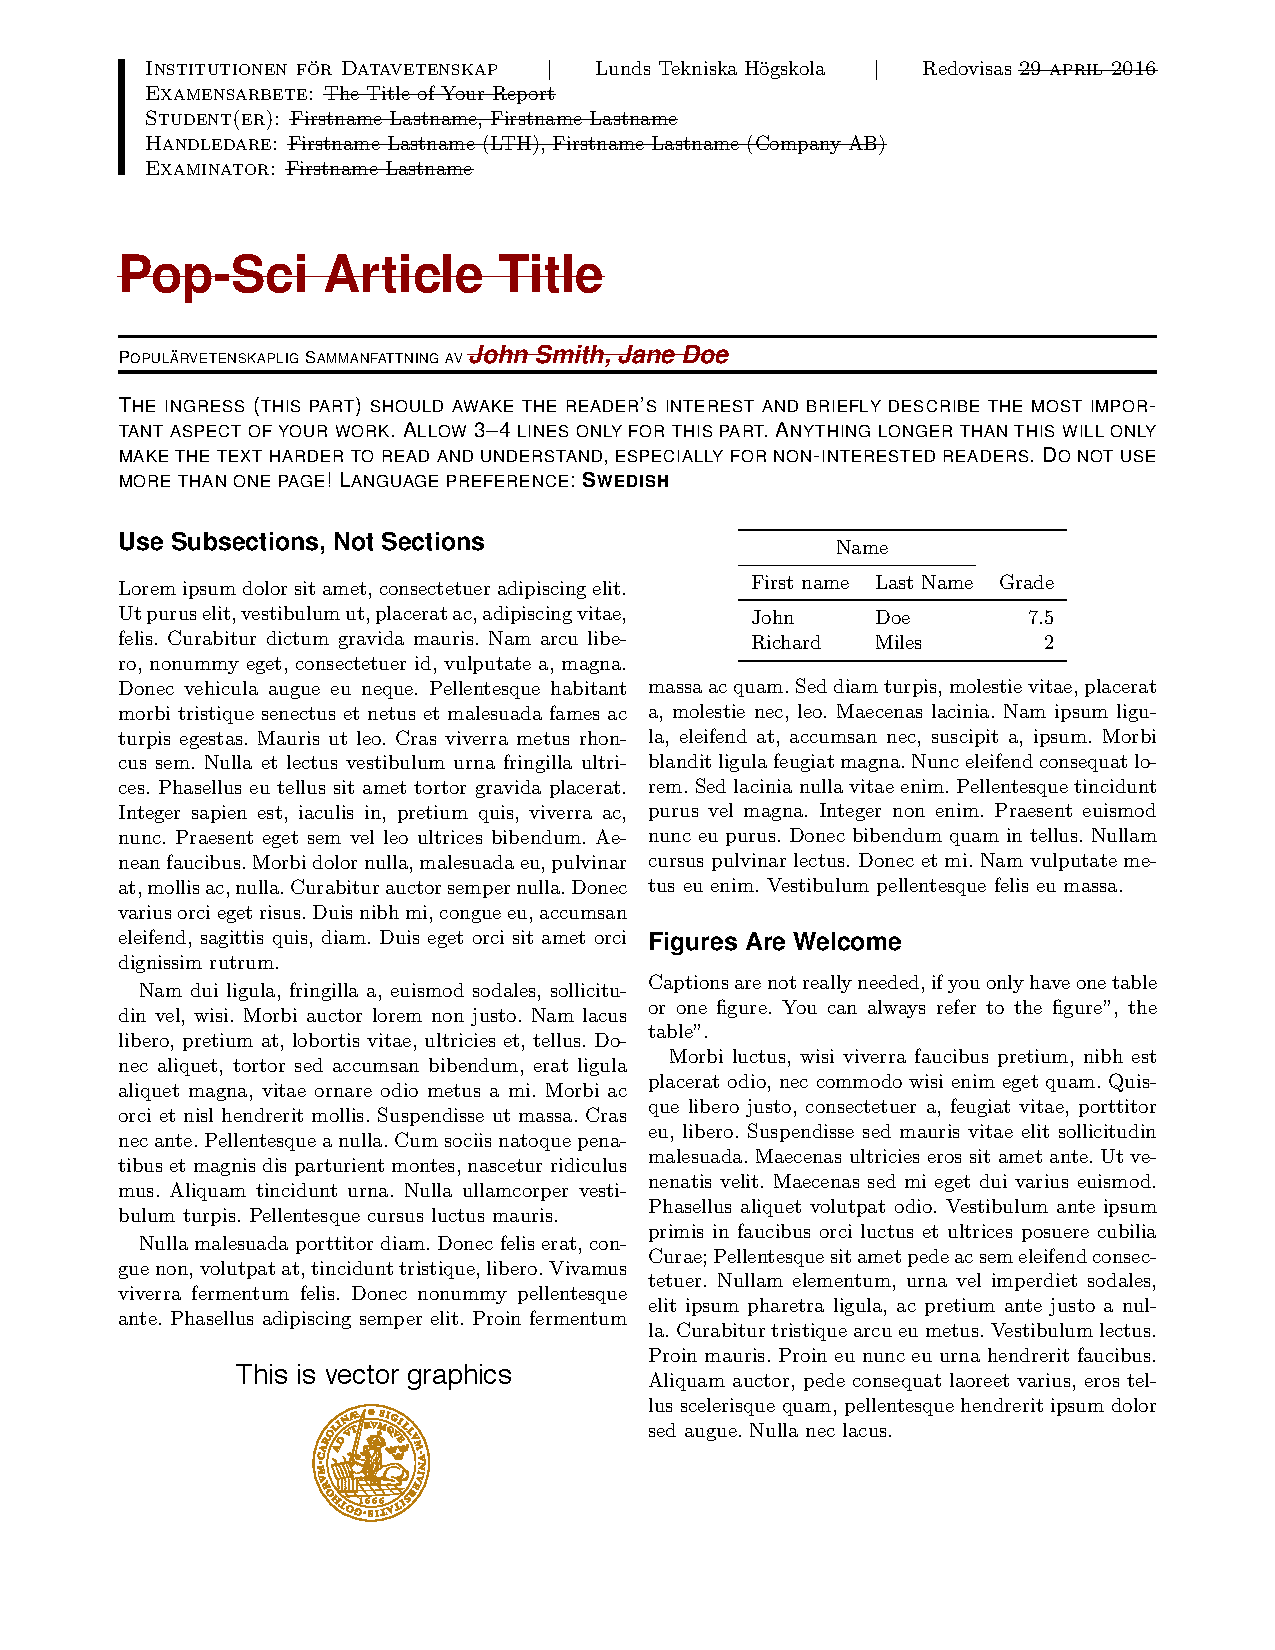
\includepdf[pages={1}]{popsci/popsci.pdf}
\end{appendices}

\end{document}
